\chapter{Kielimallien vertailu}
\label{ch:vertailu}

Eri kielimalleja löytyy erittäin paljon ja variaatioita jo pelkästään yhdestä
kielimallista voi löytyä useita variaatioita. 2025 tammikuussa hakemalla
HuggingFacesta malleja rajoituksella "Text Generation", saadaan tuloksia lähes
170 000. Tässä työssä on tuotu esille joitain jossain määrin tunnetuimmista
kielimalleista isoimmilta tekijöiltä. Kielimallien tunnettavuutta korostaa muun
muassa se, että kielimalliet esiintyvät toisten isojen kielimallien sivuilla ja
raporteissa vertailussa.

Varsinaisen toteutuksen kannalta rajoituksina on ensisijaisesti hinta. Koska
mallien toimintaa on tarkoitus vain testata, eikä ottaa pysyvään käyttöön, on
lähtökohtaisesti käytön mukaan hinnoiteltu hinnoittelu parempi. Tärkeänä
kriteerinä on myös se, että kielimallia on mahdollista saada käyttöön
kohtuullisille määrällä työtä. Näiden kriteerien myötä valituista kielimalleista
on esitelty kielimallien perustiedot, toteutustapa sovellukseen ja hinnoittelu.

\section{Google Gemini}

Gemini on Googlen julkaisema kielimalliperhe, jonka on seuraaja PaLM 2:lle
\parencite{googleKeynote2023}. Googlella on myös Gemini-niminen ChatBot, joka
tunnettiin aiemmin nimellä Bard, ennen kuin Google nimesi sen uudelleen
Geminiksi \parencite{geminiUpdates}. Geministä on useita eri malleja, jotka on
tarkoitettu eri käyttötilanteisiin. Näitä malleja ovat Ultra, Pro, Flash ja
Nano. \parencite{googleDeepmindGemini} Näistä Ultra on tarkoitettu
monimutkaisimpiin tehtäviin, Pro optimoitu kustannusten ja viiveen kannalta ja
Nano puolestaan laitteissa pyöritettäväksi
\parencite{googleDeepmindGeminiv1report}. Flash puolestaan on entistä
kustannustehokkaampi ja nopeampi kuin Pro \parencite{googleKeynote2024}.
Malleista on useita eri versioita, jotka on välillä nimetty samoin kuin
edelliset versiot \parencite{googleDeepmindGeminiv1_5report}. Kehitys on ollut
erittäin nopeaa ja versiot vanhenevat nopeasti uusien tullessa käytettäviksi.

\subsection{Käyttö}

Gemini ei ole saatavilla Googlen AI Studion kautta ilman maksullista tilausta
Suomessa \parencite{googleAiAvailableRegions}. Geminiä on kuitenkin mahdollista
käyttää Vertex AI -alustan kautta.

Vertex AI -alustan käyttöön on tarjolla kirjastoja useille eri
ohjelmointikielille \parencite{vertexAiGenerativeAiQuickstart}. Luvussa
\ref{ch:sovellus} esitellyn sovelluksen taustajärjestelmä on toteutettu Javalla
ja pakettimanagerina on maven, joten Vertex AI:n Javalle tekemän kirjasto
saadaan käyttöön lisäämällä pom.xml-tiedostoon esimerkin
\ref{lst:vertexai-pom.xml} mukaisesti.

\begin{lstlisting}[
    basicstyle=\small,
    caption={google-cloud-vertexai riippuvuus pom.xml tiedostoon},
    label={lst:vertexai-pom.xml},
    language=xml,
]
<dependency>
    <groupId>com.google.cloud</groupId>
    <artifactId>google-cloud-vertexai</artifactId>
    <version>1.2.0</version>
</dependency>
\end{lstlisting}

Kevään 2024 aikana riippuvuuteen on tullut useita versioita, joista osa on
tuonut rikkovia muutoksia \parencite{mavenGoogleVertexAIAPI}. Kirjastoon
liittyvät koodit tässä työssä on tehty versiolle 1.2.0.

VertexAI:n kirjaston käyttäminen pohjautuu VertexAI-luokasta luotavaan
ilmiintymään, jota eri mallit käyttävät. Kyseinen ilmiintymä saadaan luotua
luomalla kohdan \ref{lst:AIConfig.java} mukaisesti VertexAI-bean, jonka myötä
ilmiintymää saadaan käytettyä Spring Frameworkin avulla helposti usealla eri
paikalla ilman, että konfiguraatio tarvitsee sotkea varsinaiseen toteutukseen
\parencite{baeldungSpringBean}.

\begin{lstlisting}[
    basicstyle=\small,
    caption={VertexAI konfiguraatio},
    label={lst:AIConfig.java},
    language=java,
]
// Merkitän luokka konfiguraatioksi, jotta Spring Framework saa
// käytetyä luokassa määriteltyjä asioita
@Configuration
public class AIConfig {

    // Luetaan ympäristömuuttujista VertexAI:n tarvitsema projekti
    // tunniste
    @Value("${VERTEX_AI_PROJECT_ID}")
    private String VERTEX_AI_PROJECT_ID;

    // Luetaan ympäristömuuttujista VertexAI:n tarvitsema rajapinnan
    // sijainti tieto
    @Value("${VERTEX_AI_LOCATION}")
    private String VERTEX_AI_LOCATION;

    // Luodaan VertexAI-bean ympäristömuuttujista luetuilla tiedoilla
    @Bean
    public VertexAI vertexAI() {
        return new VertexAI(VERTEX_AI_PROJECT_ID, VERTEX_AI_LOCATION);
    }
}
\end{lstlisting}

Konfiguraation jälkeen voidaan toteuttaa varsinainen Service, jossa kielimallia
käytetään. Esimerkki tällaisesta Servicestä on esitelty kohdassa
\ref{lst:GeminiServiceExample.java}.

\begin{lstlisting}[
    basicstyle=\small,
    caption={Esimerkki toteutus siitä, miten Geminiä voisi käyttää},
    label={lst:GeminiServiceExample.java},
    language=java,
]
// Merkitään luokka Serviceksi Spring Frameworkille
@Service
@RequiredArgsConstructor
public class GeminiService {

    private final VertexAI vertexAI;

    // Luodaan kielimallille konfiguraatio
    private GenerationConfig createGenerationConfig() {
        return GenerationConfig.newBuilder()
            .setMaxOutputTokens(2000)
            .build();
    }

    public void example() {
        // Luodaan ilmiintymä mallista
        GenerativeModel model =
            new GenerativeModel("gemini-1.0-pro", vertexAI);

        // Luodaan mallista Chat-istunto, jotta mallinan kanssa
        // voidaan jatkaa keskustelua
        ChatSession chatSession = model.startChat();

        // Annetaan istunnolle konfiguraatiot
        chatSession.withGenerationConfig(createGenerationConfig());

        // Lähetetään kielimallin kanssa luotuun chat-istuntoon
        // viesti "Kerro vitsi"
        GenerateContentResponse response =
            chatSession.sendMessage("Kerro vitsi");

        // Tulostetaan kielimallin vastaus
        System.out.println(response
            .getCandidates(0).getContent()
            .getParts(0).getText());
    }
}
\end{lstlisting}

\subsection{Hinnoittelu}

Gemini 1.0 Pron hinta syötteenä annetuille kuville on \$0.0025 / kuva, videolle
\$0.002 / sekunti, tekstille \$0.000125 / 1000 merkkiä ja ulostulolle
\$0.000375 / 1000 merkkiä. Gemini 1.5 Pron hinnat ovat noin puolet syötteelle
eli kuville \$0.001315 / kuva, videoille \$0.001315 / sekunti, tekstille
\$0.00125 / 1000 merkkiä ja äänelle \$0.000125 / sekunti. Ulostulo puolestaan
on 10-kertaa kalliimpi eli \$0.00375 / 1000 merkkiä. Gemini 1.5 Pron hinnat
kaksinkertaistuvat mikäli käytössä oleva konteksti on yli 128 000. Gemini
1.5 Flashin hinnat ovat 10\% siitä mitä Gemini 1.5 Pron hinnat ovat.
\parencite{vertexAiGenerativeAiPricing} Hintoja on havainnollistettu taulukossa
\ref{tab:vertex-ai-generative-ai-pricing}.

\begin{table}[H]
  \centering
  \rowcolors{2}{gray!25}{white}
  \caption{Esimerkki hintoja eri syötteille ja ulostuloille}
  \label{tab:vertex-ai-generative-ai-pricing}
  \begin{tabular}{lccc}
    \textbf{Esimerkki} & \textbf{Gemini 1.0 Pro} & \textbf{Gemini 1.5 Pro} & \textbf{Gemini 1.5 Flash} \\
    \hline
    \Gape[0pt][2pt]{\makecell[l]{Syöte: 500 merkkiä\\Ulostulo: 1000 merkkiä}} & 0,041 snt & 0,408 snt & 0,041 snt \\
    \Gape[0pt][2pt]{\makecell[l]{Syöte: 1 kuva\\Ulostulo: 1000 merkkiä}} & 0,27 snt & 0,47 snt & 0,047 snt \\
    \Gape[0pt][2pt]{\makecell[l]{Syöte: 10 minuutin video\\Ulostulo: 1000 merkkiä}} & 1,123 € & 0,739 € & 0,074 € \\
    \Gape[0pt][2pt]{\makecell[l]{Syöte: 30 minuuttia ääntä\\Ulostulo: 1000 merkkiä}} & - & 0.213 € & 0.021 € \\
    \hline
  \end{tabular}
\end{table}

\section{PaLM 2}

PaLM:n uudempi versio, PaLM 2, on Googlen 2023 loppukeväällä julkaisema
kielimalli. Kielimallista tehtiin useampi erikokoinen malli: Gecko, Otter,
Bison ja Unicorn. Näistä pienin, Gecko, oli mitoitettu toimimaan puhelimissa ja
mahdollistamaan kielimallin käyttäminen ilman internet-yhteyttä. Näiden lisäksi
toteutettiin muun muassa lääketieteellisellä datalla hienosäädetty Med-PaLM 2.
\parencite{googleKeynote2023} \parencite{googlePaLM2Introducing}

PaLM 2:n kouluttamiseen käytettiin muun muassa verkkodokumentteja, kirjoija,
koodia, matematiikkaa ja keskusluita. PaLM 2:n koulutuksessa huomioitiin
merkittävästi paremmin useat eri kielet. \parencite{googlePaLM2TechReport}

Sittemmin muun muassa PaLM API on deprekoitu ja kehittäjiä on suositeltu
siirtymään Geminin pariin \parencite{googlePaLMAPIDeprecated}. Myös hinnoittelu
ja maininta Bison Text ja Chat -malleista on poistettu, vaikka malleja on vielä
mahdollista käyttää 2024 alkukesästä Vertex AI:n kirjastojen avulla.

\subsection{Käyttö}

PaLM 2 käyttäminen onnistuu VertexAi:n kautta vastaavasti kuin Geminin ja
tämä on esitelty kohdassa \ref{lst:PaLM2Service.java}.

\begin{lstlisting}[
    basicstyle=\small,
    caption={Esimerkki toteutus siitä, miten PaLM2:sta voisi käyttää},
    label={lst:PaLM2Service.java},
    language=java,
]
// Merkitään luokka Serviceksi Spring Frameworkille
@Service
@RequiredArgsConstructor
public class PaLM2Service {

    // Luetaan ympäristömuuttujasta
    @Value("${VERTEX_AI_PROJECT_ID}")
    private String VERTEX_AI_PROJECT_ID;

    @Value("${VERTEX_AI_LOCATION}")
    private String VERTEX_AI_LOCATION;

    @Value("${VERTEX_AI_PUBLISHER:google}")
    private String VERTEX_AI_PUBLISHER;

    private final VertexAI vertexAI;

    // Luodaan konfiguraatio kielimallille
    private com.google.protobuf.Value getParameters()
        throws InvalidProtocolBufferException, JsonProcessingException
    {
        Map<String, Object> parameters = new HashMap<>();
        parameters.put("temperature", 0.2);
        parameters.put("maxOutputTokens", 1000);
        parameters.put("topP", 0.95);
        parameters.put("topK", 40);
        return convertMapToValue(parameters);
    }

    public void example() {
        // Määritellään käytettävä päätepiste
        var endpoint =
            EndpointName.ofProjectLocationPublisherModelName(
                VERTEX_AI_PROJECT_ID,
                VERTEX_AI_LOCATION,
                VERTEX_AI_PUBLISHER,
                "text-bison"
            );

        // Muutetaan syöte haluttuun muotoon
        Map<String, Object> instance = new HashMap<>();
        instance.put("prompt", "Kerro vitsi");
        var prompt = convertMapToValue(instance);

        // Rakennetaan pyyntö
        var request = PredictRequest.newBuilder()
            // Käytetään luotua päätepistettä
            .setEndpoint(endpoint.toString())
            // Annetaan määritellyt asetukset
            .setParameters(getParameters())
            // Annetaan syöte
            .addInstances(prompt)
            .build()

        // Tehdään pyyntö
        PredictResponse predictResponse =
            vertexAI.getPredictionServiceClient().predict(request);

        // Tulostetaan vastaus
        System.out.println(predictResponse
            .getPredictions(0)
            .getStructValue()
            .getFieldsOrThrow("content")
            .getStringValue());
    }

    // Apufunktio datan muuttamiseen haluttuun muotoon
    private com.google.protobuf.Value convertMapToValue(
        Map<String, Object> map
    ) throws InvalidProtocolBufferException, JsonProcessingException {
        String json = objectMapper.writeValueAsString(map);
        com.google.protobuf.Value.Builder instanceValue =
            com.google.protobuf.Value.newBuilder();
        JsonFormat.parser().merge(json, instanceValue);
        return instanceValue.build();
    }
}
\end{lstlisting}

\section{Llama}

Llama on Meta AI:n 2023 helmikuussa esittelemä kokoelma kielimalleja
\parencite{llama1}. Llama 2 julkaistiin samana vuonna heinäkuussa
\parencite{llama2}, Llama 3 huhtikuussa 2024 \parencite{llama3} ja 3.1
heinäkuussa 2024 \parencite{llama31}. Uusimmasta versiosta 3.1 on olemassa
kolme erikokoista mallia, jotka on tarkoitettu kukin itselleen sopivaan
tarkoitukseen, 8B toimimaan kevyenä ja nopeana, 70B hinta/laatu suhteeltaan
parhaalta ja 405B toimimaan kaikista parhaiten vaihtelevissa tilanteissa
\parencite{llama}. Näiden lisäksi on julkaistu useita versioita muita malleja,
jotka on suunniteltu tiettyyn käyttötarkoitukseen kuten Llama Guard, joka
pyrkii luokittelemaan sisältöä ja määrittelemään kehotteiden ja vastausten
turvallisuutta \parencite{llamaGuard3} sekä Code Llama, joka puolestaan on
suunniteltu täydentämään koodia \parencite{llamaOtherModels}.

\subsection{Käyttö}

Vertex AI:n Model Gardenissa on ollut 23.07.2024 alkaen tarjolla Llama 3.1:sta
API Service, joka mahdollistaa Llama 3.1:n käyttämisen vastaavasti kuin
Geminin. Tämän ansiosta mallia ei tarvitse itse laittaa ajoon, jolloin laskutus
olisi tuntipohjainen vaan laskutus tapahtuu käytettyjen tokenien mukaan.
\parencite{vertexAiModelGardenLlama3}

Vertex AI:n SDK tukee valmiiksi useita eri modeleita, myös muita kuin Geminin
eri variaatioita, joten toteutus voi olla käytännössä täysin sama kuin aiemmin
esiltelty toteutus Geminin kanssa kohdassa \ref{lst:GeminiServiceExample.java}.
Luomalla oman servicen saadaan kuitenkin mukautettua sisällössä annettava ohje
sekä parametrit sopivammaksi Llama 3.1-mallille.

\subsection{Hinnoittelu}

Useat kolmannet osapuolet tarjoavat rajapinnan, jonka kautta mallia on
mahdollista käyttää ja hinnoittelu pohjautuu tokenien määrään. Halvin
ilmoitettu hinnat ja tarjoajat näkyvät taulukossa
\ref{tab:third-party-llama-prices}. Keskimääräiset hinnat esitellyille
kolmansille osapuolille ovat taulukossa \ref{tab:third-party-llama-prices-2}.
Kolmansia osapuolia ovat AWS, Azure, Databricks, Fireworks.ai, IBM, Octo.ai,
Snowflake ja Togerher.AI. \parencite{llama} Taulukko ei kata kuin vain osan
mahdollisista kolmannen osapuolen palveluntarjoajista sillä muun muassa
Vertex AI:n kautta on saatavilla myös rajapinta Llama 3.1:lle
\parencite{vertexAiModelGardenLlama3}.

\begin{table}[H]
  \centering
  \rowcolors{2}{gray!25}{white}
  \caption{Halvimmat esitellyistä kolmannen osapuolen tarjoamista rajapintojen hinnoista mallia kohden \parencite{llama}}
  \label{tab:third-party-llama-prices}
  \begin{tabular}{llcc}
    \textbf{Malli} & \textbf{Palveluntarjoaja} & \textbf{Syöttö} & \textbf{Ulostulo} \\
    \hline
    Llama 3.1 8B   & Octo.ai      & \$0.15 / MTok & \$0.15 / MTok \\
    Llama 3.1 70B  & Togerher.AI  & \$0.88 / MTok & \$0.88 / MTok \\
    Llama 3.1 405B & Fireworks.ai & \$3.00 / MTok & \$3.00 / MTok \\
    \hline
  \end{tabular}
\end{table}

\begin{table}[H]
  \centering
  \rowcolors{2}{gray!25}{white}
  \caption{Esiteltyjen kolmansien osapuolien tarjoamien rajapintojen hintojen keskiarvot mallia kohden \parencite{llama}}
  \label{tab:third-party-llama-prices-2}
  \begin{tabular}{lcc}
    \textbf{Malli} & \textbf{Syöttö} & \textbf{Ulostulo} \\
    \hline
    Llama 3.1 8B   & \$0.33 / MTok &  \$0.42 / MTok \\
    Llama 3.1 70B  & \$1.81 / MTok &  \$2.27 / MTok \\
    Llama 3.1 405B & \$5.83 / MTok & \$11.88 / MTok \\
    \hline
  \end{tabular}
\end{table}

\section{Claude}

Tekoälyn turvallisuuteen ja tutkimukseen keskittyvä yritys, Anthropic, on
luonut oman tekoälynsä, Clauden. Claude on pyritty rakentamaan
tietoturvalliseksi, luotettavaksi ja varmaksi. \parencite{anthropicCompany}
\parencite{anthropicClaude} Näihin on pyritty esimerkiksi tutkimuksien avulla,
jotka ovat keskittyneet muun muassa suojauksen murtamisen (jailbreaking)
estämiseen. \parencite{anthropicResearch}

Nykyisin Claudesta on kolme eri mallia versiolla 3.0. Näitä malleja ovat
Sonnet, Opus ja Haiku. Pääasiallisesti Opus on isoin ja paras malli kun Haiku
puolestaan keskittyy nopeuteen ja on huomattavasti pienempi. Sonnet puolestaan
jää näiden kahden välimaastoon. Sonnetista on kuitenkin julkaistu uudempi
versio 3.5, joka on saatu Opus:ta paremmaksi kuitenkin pitäen kulut samana kuin
3.0 versiossa. Tilannetta on havainnollistettu kuvassa
\ref{fig:3-5-sonnet-curve}. \parencite{anthropicAPIDocsModels}

\begin{figure}[H]
  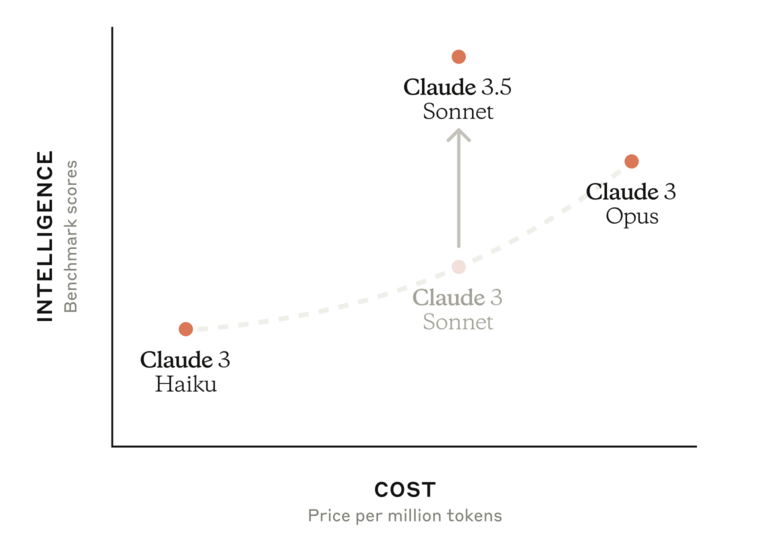
\includegraphics[width=\textwidth]{figures/3-5-sonnet-curve.png}
  \caption{Anthropic API dokumentaatiossa oleva havannollistava kuva mallien eroista 05.08.2024}
  \label{fig:3-5-sonnet-curve}
\end{figure}

Claudea on mahdollista kokeilla web-käyttöliittymän kautta rekisteröitymisen
jälkeen ilmaisena muutamia kyselyitä päivässä \parencite{claudeChat}. Tarjolla
on myös Anthropic API, joka vaatii aktiivisen tilauksen. APIa voi käyttää
tarjolla olevien kirjastojen avulla tai vaihtoehtoisesti suorittaa itse kutsuja
API-dokumentaation mukaisesti. Claude on saatavilla myös AWS Bedrockin sekä
Vertex AI:n kautta. \parencite{anthropicAPIDocs}

\subsection{Käyttö}
\label{ch:claude-usage}

Anthropic tarjoaa vain python kirjastoja Clauden käyttöön, joten sovellukseen
integrointi tehdään kutsuen suoraan saatavilla olevaa rajapintaa. Yksi
yksinkertainen vaihtoehto on käyttää openfeign:iä, joka saadaan käyttöön
lisäämällä `pom.xml`:n riippuvuuksiin \ref{lst:openfeign-pom.xml} mukainen
riippuvuus.

\begin{lstlisting}[
    basicstyle=\small,
    caption={spring-cloud-starter-openfeign riippuvuus pom.xml tiedostoon},
    label={lst:openfeign-pom.xml},
    language=xml,
]
<dependency>
    <groupId>org.springframework.cloud</groupId>
    <artifactId>spring-cloud-starter-openfeign</artifactId>
    <version>4.1.3</version>
</dependency>
\end{lstlisting}

Openfeign riippuvuuden lisäämisen jälkeen saadaan määritään kohdassa
\ref{lst:ClaudeConfig.java} oleva konfiguraatio, jotta saadaan jokaiseen
pyyntöön lisätty otsikkotietoihin API-avain ja versio, joita rajapinnan
käyttämisen vaatii \parencite{anthropicAPIDocsVersions}
\parencite{anthropicAPIDocsGettingStarted}.

\begin{lstlisting}[
    basicstyle=\small,
    caption={Konfiguraation Claude:lle luodulle Openfeign clientille},
    label={lst:ClaudeConfig.java},
    language=java,
]
public class ClaudeConfig {

    // Luetaan ympäristömuuttujista API avain
    @Value("${CLAUDE_API_KEY}")
    private String CLAUDE_API_KEY;

    @Bean
    public RequestInterceptor requestInterceptor(){
        // Lisätään käytettävä versio ja API avain pyyntöjen
        // otsikkotietoihin
        return requestTemplate -> {
            requestTemplate.header("anthropic-version", "2023-06-01");
            requestTemplate.header("x-api-key", CLAUDE_API_KEY);
        };
    }
}
\end{lstlisting}

Tämän jälkeen määritellään interface, josta OpenFeign luo käytettävän clientin.
Kyseinen interface on nähtävissä kohdassa \ref{lst:ClaudeApiClient.java}.

\begin{lstlisting}[
    basicstyle=\small,
    caption={Konfiguraation Claude:lle luodulle Openfeign clientille},
    label={lst:ClaudeApiClient.java},
    language=java,
]
// Kerrotaan OpenFeign:lle, että tämän interfacen perusteella tulee
// luoda toteutus Claude rajapinnalle
@FeignClient(
    name = "claude-api",
    url = "https://api.anthropic.com/v1/",
    configuration = ClaudeConfig.class
)
public interface ClaudeApiClient {

    // Määritellään mahdolliset pyynnöt

    @PostMapping("messages")
    MessagesResponse messages(@RequestBody MessagesRequest messagesRequest);
}
\end{lstlisting}

OpenFeign luo määritellyn interfacen pohjalta automaattisesti ilmiintymän, jota
voidaan käyttää kohdan \ref{lst:ClaudeService.java} mukaisesti.

\begin{lstlisting}[
    basicstyle=\small,
    caption={Konfiguraation Claude:lle luodulle Openfeign clientille},
    label={lst:ClaudeService.java},
    language=java,
]
// Merkitään luokka Serviceksi Spring Frameworkille
@Service
@RequiredArgsConstructor
public class ClaudeService {

    // OpenFeign luo automaattisesti ilmiintymän, jonka Spring
    // Framework alustaa tähän muuttujaan
    private final ClaudeApiClient claudeApiClient;

    public void example() {
        // Luodaan pyyntö
        var request = new MessagesRequest(new Message("user", "Hello world!"));
        // Tehdään pyyntö
        var response = claudeApiClient.messages(request);

        // Tässä voidaan käsitellä saatu vastaus miten halutaan
    }
}
\end{lstlisting}

\subsection{Hinnoittelu}

Clauden hinnoittelu vaihtelee hiukan sivuston mukaan. Claude.ai:n Pro-tilauksen
hinnoiksi ilmoitetaan \$20 tai 18€ + ALV ja Team-tilaukselle \$25/\$30 tai
23€/28€ + ALV. \parencite{anthropicPricing} \parencite{claudePricing} Anthropic
API:n hinnat on esitetty taulukossa \ref{tab:anthropic-api-pricing}

\begin{table}[H]
  \centering
  \rowcolors{2}{gray!25}{white}
  \caption{Anthropic APIn hinnat}
  \label{tab:anthropic-api-pricing}
  \begin{tabular}{lcc}
    \textbf{Malli} & \textbf{Syöttö} & \textbf{Ulostulo} \\
    \hline
    Claude 3.5 Sonnect &    \$3 / MTok &   \$15 / MTok \\
    Claude 3 Opus      &   \$15 / MTok &   \$75 / MTok \\
    Claude 3 Haiku     & \$0.25 / MTok & \$1.25 / MTok \\
    \hline
  \end{tabular}
\end{table}

Clauden ilmainen tilaus sisältää vain Claude 3.5 Sonnetin käyttämisen web-
käyttöliittymän sekä sovellusten kautta. Pro-tilaus lisää mahdollisuuden
käyttää Opus- ja Haiku-malleja sekä joitain QoL-lisäyksiä ja suurempaa
prioriteettia käyttäjälle. Team-tilaus on lähinnä tiimin hallinnan ja maksun
kannalta oleellisia lisätoiminnallisuuksia. Pro-tilaus lisää viisin kertaisen
käyttörajan verrattuna ilmaiseen ja Team-tilaus sitäkin suuremman.
\parencite{anthropicPricing} \parencite{claudePricing} Selviä käyttörajoja ei
ole saatavilla.

\section{xAI}

XAi on Elon Muskin johtama tekoälyritys, joka on luonut Grok-kielimallin
\parencite{xAIAbout}. Grok kielimallin on epäilty olevan vain yksi kielimalli
lisää muiden joukossa \parencite{fireshipElonsGrokAI}, jonka perustamisen
taustalla vaikuttaa olevan ennemminkin huumoriset päähänpistokset
\parencite{twitter1679182035645235200} ja erimielisyydet ja oikeusjutut
muun muassa OpenAI:n kanssa, jonka perustajistoon Elon Musk kuuluu
\parencite{fireshipElonsLawsuitAgainstOpenAI}.

Marraskuussa 2024 Grok kielimallille avattiin rajapinta, jota kehittäjät
pääsevät kokeilemaan vähintään vuoden 2024 loppuun asti. Jokaiselle
rekisteröityneelle annetaan ilmaista kredittiä 25 dollarin verran
kuukaudessa. Rajapinta on toteuttu yhteensopivaksi OpenAI:n ja Anthropicin
tarjoamien rajapintojen kanssa, joka mahdollistaa jo tehtyjen toteutuksien
erittäin helpon vaihtamisen käyttämään xAI:n rajapintaa. \parencite{xAIBlogApi}

\subsection{Käyttö}

Dokumentaatiossa luetellut integraatiot pohjautuvat olemassa oleviin OpenAI:n
ja Anthropic SDK:oihin, jotka on toteutettu JavaScriptille ja Pythonille
\parencite{xAIDocsIntegrations}. Näiden käyttö ei tällöin onnistu suoraan
työn ohella tehdyn sovelluksen kanssa, joten toteutus tulee tehdä tarjolla
olevan REST-rajapinnan kautta, kuten luvussa \ref{ch:claude-usage} tehtiin
Clauden kanssa.

Saamme API-avaimen määriteltyä dokumentaation mukaisesti otsikkotietoihin
kohdassa \ref{lst:XAIConfig.java} esitellyllä tavalla.

\begin{lstlisting}[
    basicstyle=\small,
    caption={Konfiguraation xAI:lle luodulle Openfeign clientille},
    label={lst:XAIConfig.java},
    language=java,
]
public class XAIConfig {

    // Luetaan api avain ympäristömuuttujista
    @Value("${XAI_API_KEY:}")
    private String XAI_API_KEY;

    @Bean
    public RequestInterceptor requestInterceptor() {
        // Lisätään API-avain Authorization-otsikkotietoon
        return requestTemplate -> requestTemplate
            .header("Authorization", "Bearer " + GROK_API_KEY);
    }
}
\end{lstlisting}

Tämän jälkeen määritellään interface, josta OpenFeign luo käytettävän clientin.
Kyseinen interface on nähtävissä kohdassa \ref{lst:XAIApiClient.java}.

\begin{lstlisting}[
    basicstyle=\small,
    caption={Interface xAI:n rajapinnasta},
    label={lst:XAIApiClient.java},
    language=java,
]
// Kerrotaan OpenFeign:lle, että tämän interfacen perusteella tulee
// luoda toteutus xAI rajapinnasta
@FeignClient(
    name = "xai-api",
    url = "https://api.x.ai/v1/",
    configuration = XAIConfig.class
)
public interface XAIApiClient {

    // Määritellään mahdolliset pyynnöt

    @PostMapping("chat/completions")
    ChatCompletionsResponse chatCompletions(
        @RequestBody ChatCompletionsRequest chatCompletionsRequest
    );
}
\end{lstlisting}

OpenFeign luo määritellyn interfacen pohjalta automaattisesti ilmiintymän, jota
voidaan käyttää kohdan \ref{lst:XAIService.java} mukaisesti.

\begin{lstlisting}[
    basicstyle=\small,
    caption={Service, jossa varsinanen rajapinnan kutsuminen tapahtuu},
    label={lst:XAIService.java},
    language=java,
]
// Merkitään luokka Serviceksi Spring Frameworkille
@Service
@RequiredArgsConstructor
public class GrokService {

    // OpenFeign luo automaattisesti ilmiintymän, jonka Spring
    // Framework alustaa tähän muuttujaan
    private final GrokApiClient grokApiClient;

    public void example() {
        // Alustetaan keskustelu
        List<Message> messages = new ArrayList<>();
        messages.add(new Message("system", "Kerrot vitsejä käyttäjän antamista aiheista"));
        messages.add(new Message("user", "omena"));

        // Luodaan pyyntö keskustelun pohjalta
        ChatCompletionsRequest request =
            new ChatCompletionsRequest("grok-beta", messages);

        // Kutsutaan rajapintaa luodulla pyynnöllä
        ChatCompletionsResponse response =
            grokApiClient.chatCompletions(request);

        // Tulostetaan vastaus
        System.out.println(
            response.choices().getFirst().message().content());
    }
}
\end{lstlisting}

\subsection{Hinnoittelu}

XAI:n rajapinnan hinnoittelua ei ole avattu julkisilla sivuilla, mutta
rekisteröitymällä osaksi uuden rajapinnan julkista betaohjelmaa pääsee näkemään
eri mallien hinnoittelut ja rajoitukset. Nämä hinnat on koottu taulukkoon
\ref{tab:grok-prices} joulukuussa 2024.

\begin{table}[H]
    \centering
    \rowcolors{2}{gray!25}{white}
    \caption{xAI:n tarjomien kielimallien hinnat joulukuussa 2024}
    \label{tab:grok-prices}
    \begin{tabular}{llcc}
        \textbf{Malli} & \textbf{Syöttö (teksti)} & \textbf{Syöttö (kuva)} & \textbf{Ulostulo} \\
        \hline
        grok-beta          & \$5.00 / MTok &             - & \$15.00 / MTok \\
        grok-vision-beta   & \$5.00 / MTok & \$5.00 / MTok & \$15.00 / MTok \\
        grok-2-vision-1212 & \$2.00 / MTok & \$2.00 / MTok & \$10.00 / MTok \\
        grok-2-1212        & \$2.00 / MTok &             - & \$10.00 / MTok \\
        \hline
    \end{tabular}
\end{table}

Vastaavat tiedot malleista ja hinnoista saa haettua myös xAI:n rajapinnan
tarjoamasta päätepisteestä. \parencite{xAIDocsEndpoints}

\section{Sovellukseen valittavat kielimallit}

Aiemmin määriteltyjen ehtojen mukaisesti, on sovellukseen valittavissa
kielimalleissa ensisijaisena vaatimuksena hinnoittelu ja toisena kohtuullinen
tapa toteuttaa. Esitellyistä kielimalleista kaikki olivat mahdollista toteuttaa
kohtuullisesti, joten käytännössä vain hinta ratkaisee.

Esitellyistä kielimalleista Claude vaatii erillisen tilauksen, jotta se
voitaisiin integroida sovellukseen eikä tarjoa käytönmukaista hinnoittelua tai
vaihtoehtoisesti tarjoa kokeilujaksoa tai -krediittejä. VertexAI:n ansiosta
saadaan integroitua Gemini, PaLM 2 ja Llama käytännössä yhdellä toteutuksella,
joten ei ole syytä olla integroimatta niistä jotain kun integroidaan yksikin.
Sovellukseen tehdään tuki useille kielimalleilla, jotta niitä voidaan kokeilla
varsinaisessa käytössä, joten ei ole myöskään syytä olla integroimatta xAI:ta
osaksi sovellusta. Sovellukseen valittuja kielimalleja ovat siis Gemini,
PaLM 2, Llama ja xAI. Jokaisesta kielimallista valitaan tekohetkellä
kielimallien uusin versio ja dokumentaation peruskäyttöön suosittelema
variaatio, mikäli kielimallista on useita variaatioita.
